%\VignetteIndexEntry{The Containers Package}
%\VignettePackage{Containers}
\documentclass[10pt]{article}
\usepackage{graphicx}
\title{The Containers Package}
\author{John Hughes}
\usepackage{Sweave}
\begin{document}
\maketitle
This package furnishes R with a suite of object-oriented data structures: stack, queue, deque, max-heap, min-heap, binary search tree, and splay tree. Each R class is backed by a Java class, which means that the R type(s) of a given container's elements must map (easily) to a Java type(s) in order for use of the container to be intuitive for the typical R programmer. All of the code examples use integers, and R's double, logical, character, and vector types are also handled transparently by (most of) the containers. One caveat is worth mentioning: the internally ordered containers, i.e., the heaps and the binary search trees, do not support elements of type vector. All containers except the binary search trees offer (constant) external iterators, and the search trees offer internal iterators for in-order traversal. The diagram below shows the Containers class hierarchy.\bigskip

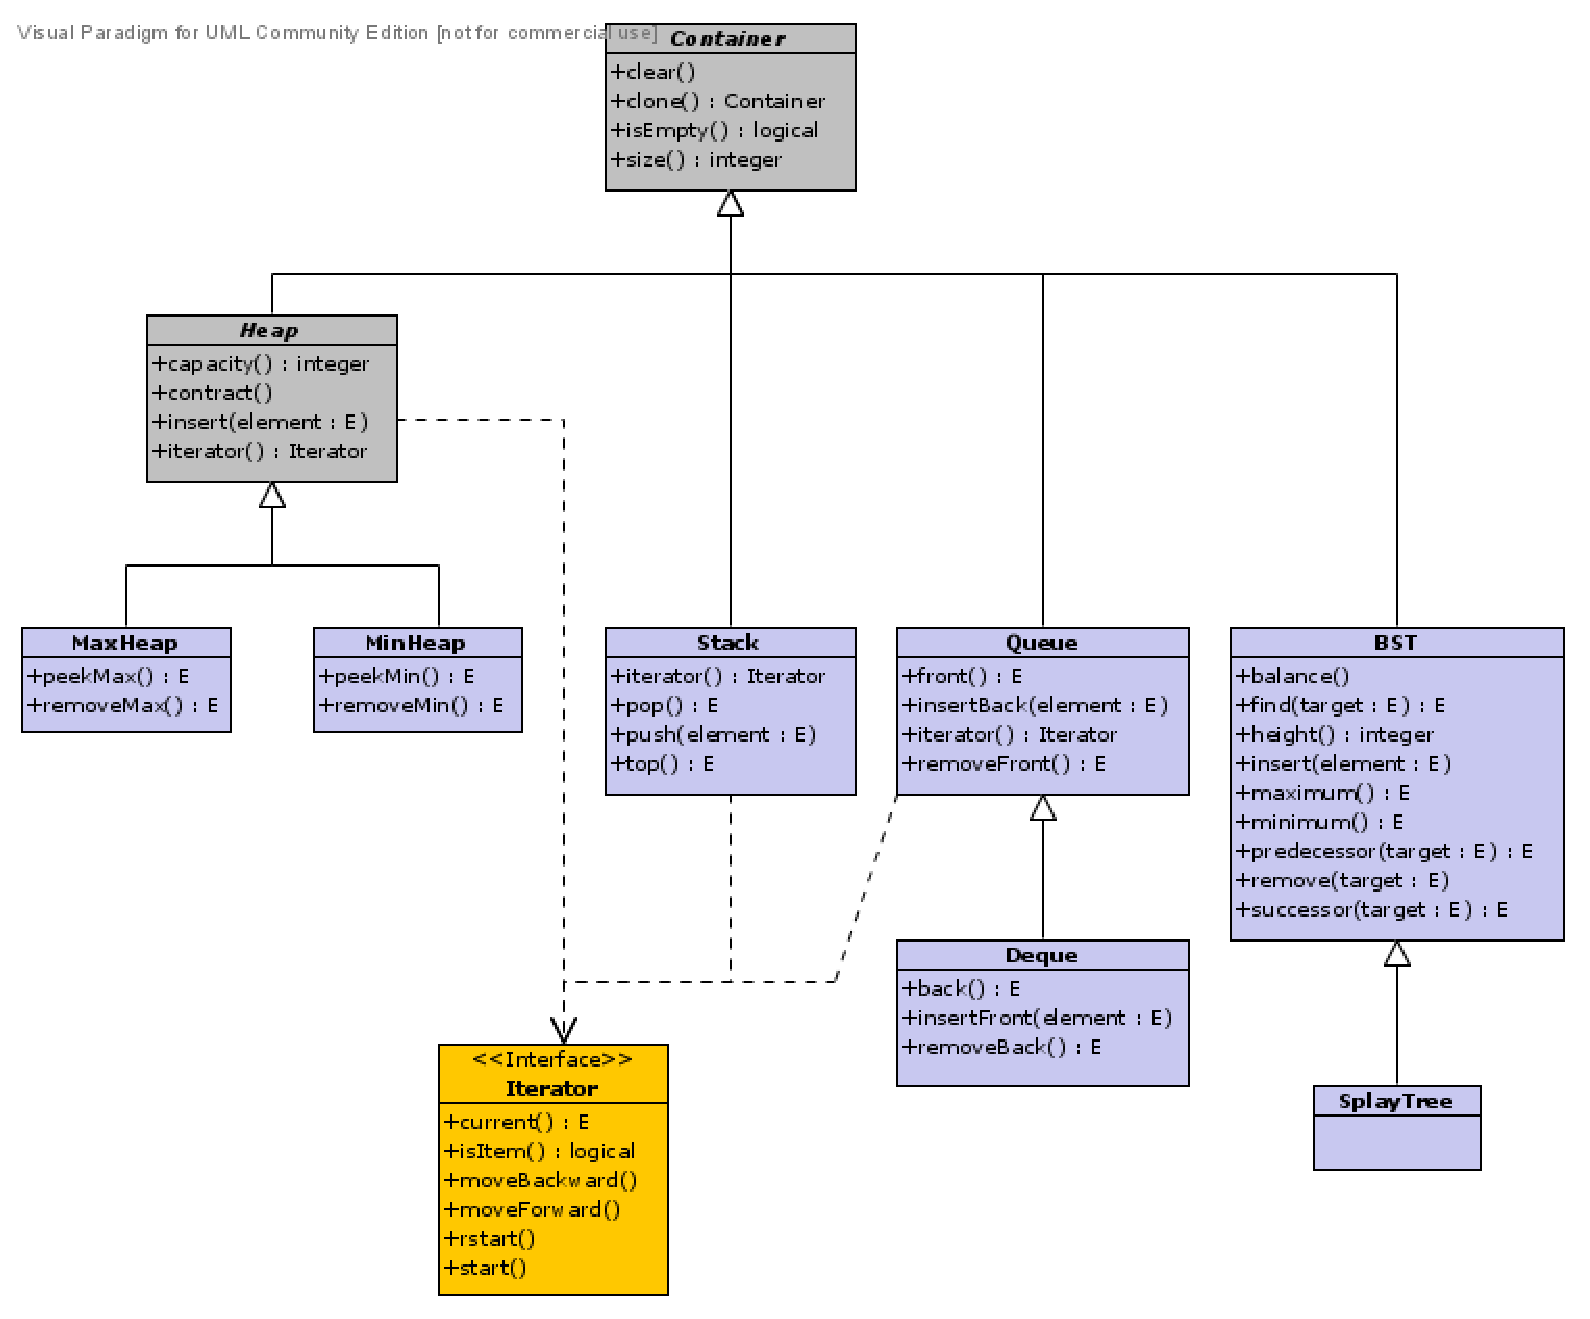
\includegraphics[scale=1]{Containers.eps}
\end{document}
